% Auteur\,: Steve Prud’Homme
% Cette oeuvre, création, site ou texte est sous licence Creative Commons Attribution - Pas d’Utilisation Commerciale - Partage dans les Mêmes Conditions 4.0 International. Pour accéder à une copie de cette licence, merci de vous rendre à l'adresse suivante 
% http://creativecommons.org/licenses/by-nc-sa/4.0/ ou envoyez un courrier à 
% Creative Commons, 444 Castro Street, Suite 900, Mountain View, California, 94041, USA.

%\,:::SNIPET
%\,::: SECTION
% \section{Contexte} 
%		\begin{frame}[allowframebreaks]
%			\frametitle{}
%			\begin {itemize}
%				\item 
%			\end{itemize}
%		\end{frame}
%:::WATER MARK / FILIGRANE
%\usepackage{draftwatermark}
%\SetWatermarkLightness{0.5}
%\SetWatermarkAngle{25}
%\SetWatermarkScale{0.5}
%\SetWatermarkFontSize{2cm}
%\SetWatermarkText{Document de travail}
%:::BIBLIOGRAPHIE NON-CITÉ
%\nocite


\documentclass{beamer}
\usepackage{color}
\usepackage{beamerthemesplit} % new 
\usepackage[french]{babel}
\usepackage[utf8]{inputenc}
\usepackage{tikz}
\usepackage[fixlanguage]{babelbib}
\selectbiblanguage{french}
% Natlib pour la bibliographie
\usepackage{natbib}
\usepackage{url}
\usetikzlibrary{mindmap,shadows,shapes,backgrounds}
\usepackage[T1]{fontenc}
\setbeamertemplate{bibliography item}[text]
\usepackage{multicol}


\definecolor{MightySlate}{RGB}{85,98,112}
\definecolor{Pacifica}{RGB}{78,205,196}
\definecolor{AppleChic}{RGB}{199,244,100}
\definecolor{CheeryPink}{RGB}{255,107,107}

\setbeamercolor{titlelike}{parent=structure}
\setbeamerfont*{title}{size=\huge}
\setbeamercolor{title}{bg=MightySlate, fg=white}
\setbeamercolor{author}{bg=Pacifica, fg=white}
\setbeamercolor{institute}{bg=AppleChic, fg=black}
\setbeamercolor{date}{bg=CheeryPink, fg=white}

\definecolor{DTUred}{RGB}{178,20,20}
\setbeamercolor*{palette primary}{use=structure,fg=white,bg=MightySlate}
\usepackage{helvet}
\usepackage{draftwatermark}
\SetWatermarkLightness{0.5}
\SetWatermarkAngle{25}
\SetWatermarkScale{0.5}
\SetWatermarkFontSize{2cm}
\SetWatermarkText{Document de travail}

\begin{document}
	\title{Plan d’action de conception et réalisation de projets de formation en ligne} 
	\subtitle{Évaluation}
	\author{Steve Prud'Homme} 
	\institute{Commission scolaire de Laval} 
	\date{\today} 

	
	%\usebackgroundtemplate{%
  %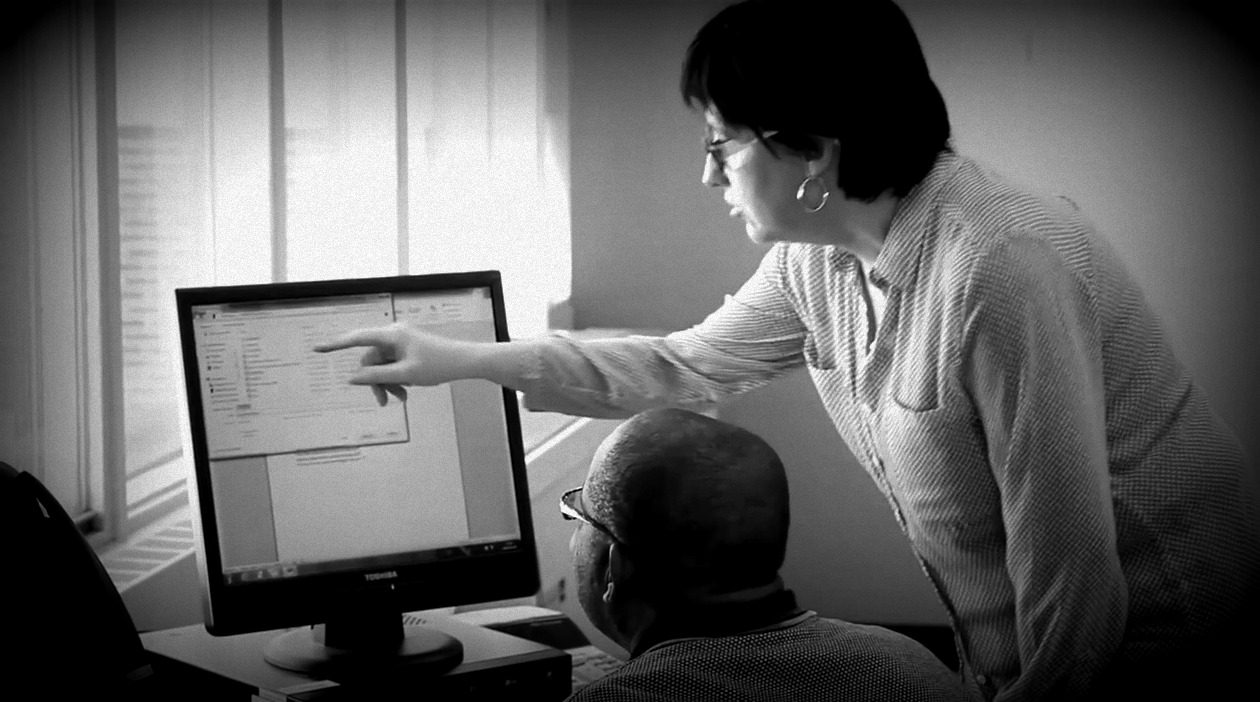
\includegraphics[height=\paperheight]{back.png}} 
	
	\frame{\titlepage} 
    
	\usebackgroundtemplate{ } 
	\par L’intention de ce document est de respecter pleinement les droits des créateurs des ressources
utilisées.
	\par En ce qui concerne les citations insérées selon le principe de l'utilisation équitable ou avec la permission de l'auteur, veuillez les contacter ou respecter les droits d’utilisation précisés dans les documents d’origine avant de les réutiliser.
	\par Si vous estimez que certains éléments de ce rapport ne respectent pas intégralement les droits de vos
publications, veuillez nous en aviser afin que les modifications nécessaires puissent être apportées au\,: \url{mailto:sprudhomme@cslaval.qc.ca}.
	\par Cette \oe uvre, création, site ou texte est sous licence Creative Commons Attribution\,-\,Pas d’Utilisation Commerciale\,-\,Partage dans les Mêmes Conditions 4.0 International.	\section{Sommaire} 
		\begin{frame}
			Cette présentation vise à\,:
			\frametitle{Sommaire}
			\begin {itemize}
				\item \textbf{Familiariser} l'auditoire sur les des situations de travail, les processus de production, 
du contrôle de la qualité et  les  bonnes pratiques en conception et réalisation d’outils pédagogiques en ligne en présentant un bref aperçu de la \textbf{littérature} et de notre survol.
				\item Démontrer qu'il est pertinent d'adopter des \textbf{pratiques harmonisées}.
				\item Promouvoir l'idée qu'il serait pertinent de \textbf{concevoir une norme, accréditation ou un cadre de référence en ce qui concerne conception et réalisation d’outils pédagogiques en ligne}.

			\end{itemize}
		\end{frame}
	\frame[allowframebreaks]{\frametitle{Ordre du jour}\tableofcontents}


	\section{Préparation du test} 
	
		
		
	\subsection{Identifier la cible utilisateur et ses caractéristiques} 
		\begin{frame}[allowframebreaks]
		\frametitle{Identifier la cible utilisateur et ses caractéristiques}
			\begin {itemize}
				      \item Qui est la clientèle cible ?
				      \item Catégorie socioprofessionnelle
					\item Âge
					\item Expérience internet
					\item Expérience avec l’outil informatique
					\item Caractéristiques particulières
			\end{itemize}
		\end{frame} 
		
	\subsection{Identifier les objectifs des utilisateurs} 
		\begin{frame}[allowframebreaks]
		\frametitle{Identifier les objectifs des utilisateurs}
		Ce demander ce que les utilisateurs de cette formation pourront faire :
			\begin {itemize}
				\item Est-ce que les les utilisateurs s’inscriront en ligne ?
				\item Est-ce que les utilisateurs auront accès à un environnement d’apprentissage
				\item Mode asychrone, synchrone ou hybride
				\item Est-ce qu'il y a des documents d’accompagnement
				\begin {itemize}
					\item Guide des apprentissages
					\item Guide des activités
					\item Journal de bord
					\item Feuille de route
				\end{itemize}
					\item Est-ce que les utilisateurs se rencontreront par visioconférence ?

			\end{itemize}
		\end{frame}
		
	\subsubsection{Identifier les tâches des utilisateurs} 
		\begin{frame}[allowframebreaks]
			\begin {itemize}
			\frametitle{Identifier les tâches des utilisateurs}
				      \item Les objectifs des utilisateurs
						\begin {itemize}
						\item Exemple : \textit{Répondre aux besoins de formation sur des fonctions spécifiques du logiciel Microsoft Word exprimés par les employés de soutien et le Service des ressources humaines.}
						\end{itemize}
					\item Définir les tâches des utilisateurs et leur importance respective dans la réalisation de chacun des objectifs.
						\begin {itemize}
						\item Exemple : \textit{mettre un exemple ici}
						\end{itemize}
					
					\end{itemize}
		\end{frame}    
	\subsubsection{Choisir les tâches que l’on va évaluer} 
		\begin{frame}[allowframebreaks]
		\frametitle{Choisir les tâches que l’on va évaluer}
			Choisir les tâches que l’on va évaluer. Par exemple :
			\begin {itemize}
				     		\item \textit{S’authentifier sur l’environnement numérique d’apprentissage.}
						\item \textit{Consulter d’un paquetage SCORM.}
						\item \textit{Répondre au questionnaire final d’un paquetage SCORM.}
						\item \textit{Répondre au formulaire d’évaluation du cours.}
						\item \textit{Être en mesure de faire le suivi de ses apprentissages.}
			\end{itemize}
		\end{frame}  
		
	\subsection{Recruter et prendre rendez-vous avec les utilisateurs} 
		
			\subsubsection{Échantillonnage} 
			
			\begin{frame}[allowframebreaks]
			\frametitle{Échantillonnage}
			Échantillonnage. Recruter des participants :
					\begin {itemize}
					\item en fonction de l’analyse de la population cible, 
					\item de niveaux variés, de tranches d’âges différentes et de genres différents.
					\end{itemize}
			\end{frame} 	
			
			\subsubsection{Le recrutement dans le processus du test utilisateur} 
			
			\begin{frame}[allowframebreaks]
			\frametitle{Le recrutement dans le processus du test utilisateur}
			\begin {itemize}
					\item La courtoisie veut que l’on contacte les participants au moins 15 jours avant le début des tests (il s’agit d’une des premières choses à effectuer).
					\item Lors de sa présentation aux participants potentiels, le test doit être dédramatisé : ce n’est pas une expérience sordide, mais plutôt une sorte de jeu, un essai d’un cours.
					\end{itemize}
			\end{frame} 
			
			\subsubsection{Combien de participants ?} 
			\begin{frame}[allowframebreaks]
			\frametitle{Combien de participants ?}
				\begin {itemize}
				\item Selon les auteurs entre 5 et 15 utilisateurs permettent de cerner la plupart des problèmes principaux de convivialité \citep{nielsen1993a}\citep{spool2001a} \citep{cockton2008a} 
				\item \textit{... of the randomly selectedsets of 5 participants found
99\% of the problems; other sets found only 55\%. With 10 users, the lowest percentage of problems revealed
by any one set was increased to 80\%, and with 20 users, to 95\%.}  \citep{cockton2008a}
				\item Un consensus semble se faire autour de 8 à 10 utilisateurs. On considère que c'est la plupart du temps un compromis raisonnable entre coût de l'intervention et résultats obtenus.  \citep{ergolab2014a}
				\end{itemize} 
			\end{frame} 
			
			
			\subsubsection{Le plan de test} 
			\begin{frame}[allowframebreaks]
			\frametitle{Le plan de test}
				Le plan de test est constitué :
				\begin{itemize}
				\item d’une liste de questions, 
				\item de scénarios, 
				\item de points-clés que l’on doit explorer pendant le test.
				\end{itemize} 
				\framebreak
				\begin{itemize}
				\item Il consiste à \textbf{décrire de façon détaillée} les scénarios de navigation permettant d’évaluer les tâches-clés, ou de délimiter la partie de l’application/du site web pour laquelle on prévoit une navigation libre.
				\item Le scénario peut être rendu plus crédible lorsqu’il réunit plusieurs questions, afin de simuler une véritable activité de l’utilisateur sur le site.
				\item Étapes de recueil de descriptions subjectives de l’expérience (concernant la réalisation d’une tâche en particulier ou de la navigation globale dans le site).
				\end{itemize} 
				\end{frame} 
				
		\subsubsection{Le plan de test} 
			\begin{frame}[allowframebreaks]
			\frametitle{Le plan de test}
				Le plan de test est constitué :
				\begin{itemize}
				\item d’une liste de questions, 
				\item de scénarios, 
				\item de points-clés que l’on doit explorer pendant le test.
				\end{itemize} 
				\framebreak
				\begin {itemize}
				\item Il consiste à \textbf{décrire de façon détaillée} les scénarios de navigation permettant d’évaluer les tâches-clés, ou de délimiter la partie de l’application/du site web pour laquelle on prévoit une navigation libre.
				\item Le scénario peut être rendu plus crédible lorsqu’il réunit plusieurs questions, afin de simuler une véritable activité de l’utilisateur sur le site.
				\item Étapes de recueil de descriptions subjectives de l’expérience (concernant la réalisation d’une tâche en particulier ou de la navigation globale dans le site).
				\end{itemize} 
						
				
			\end{frame} 
			
			\subsubsection{Type de protocole} 
			\begin{frame}[allowframebreaks]
			\frametitle{Type de protocole }
				Le choix d'un protocole écrit ou oral est souvent lié aux préférences et à ses convictions concernant les façons « idéales » de conduire un test.

				\begin{itemize}
				\item Le protocole écrit permet :
					\begin{itemize}
					\item de conserver une distance à l'utilisateur,
					\item de présenter des risques d'être mal interprété,
					\item de mettre l'utilisateur mal à l'aise à cause de la rigueur qu'il introduit,
					\item d'éloigner le participant d'une situation potentiellement réelle d'utilisation. 
					\end{itemize} 
				\framebreak
				\item Le protocole oral permet :
				\begin{itemize}
					\item d'orienter le test vers une dimension plus réaliste et humaine,
					\item d'entraîner des questions de la part de l'utilisateur,
					\item le risque d'influencer l'utilisateur dans ses réponses à causes des réponses à ses questions,
					\item de travailler dans avec grande rigueur puisque les scénarios doivent toujours être proposés de la même manière . 
					\end{itemize} 
				\end{itemize} 
				\end{frame} 
				
				
				
			\subsubsection{Durée du test} 
			\begin{frame}[allowframebreaks]
			\frametitle{Durée du test}
				

				\begin{itemize}
				\item Pas plus d'une heure (fonctionnement attentionnel)
				\item Plus long si on introduit une pause. 	
				\end{itemize} 
				\end{frame} 	
				
				
				
					   
					
		
		
	\subsection{Préparer préquestionnaire et postquestionnaires} 
		
		\subsubsection{Préquestionnaire}
		\begin{frame}[allowframebreaks]
		\frametitle{Préquestionnaire}
			Il s'agit d'une entrée en matière. Il permet :
			\begin {itemize}
				      \item d'introduire l'utilisateur au test,
				      \item de recueillir des informations de base, 
				      \item d'obtenir l'accord du participant si l'on envisage de le filmer,
				      \item de sélectionner des participants représentatifs de la cible finale s'il est administré avant même de recruter les utilisateurs,
				      \item de déterminer le niveau d'expertise de l'utilisateur, c'est à dire :
				      \begin {itemize}
				      \item l'expertise informatique
				      \item l'expertise de la navigation sur internet, 
				      \item l'expérience de l'application, 
				      \item l'expertise concernant la tâche principale supportée par l'application,
				      \item l'expertise métier ;
				      \end{itemize}
				      \item de déterminer la durée et fréquence des utilisations.


			\end{itemize}
		\end{frame}
		
		\subsubsection{Postquestionnaires}
		\begin{frame}[allowframebreaks]
		\frametitle{Postquestionnaires}
			Il permet :
			\begin {itemize}
				      \item De recueillir des données globales sur la passation, et notamment le ressenti subjectif. 
				      \item D'expliquer certaines phases du test. 
			\end{itemize}
		\end{frame}
		
	\subsection{Préparer le plan de test en fonction des objectifs d'utilisabilité} 
	\subsubsection{Les objectifs d'utilisabilité : critères à évaluer} 

		\begin{frame}[allowframebreaks]
			\frametitle{Les objectifs d'utilisabilité : critères à évaluer}
			Il faut se baser sur des objectifs d'utilisabilité qualitatifs et quantitatifs. (par exemple 100\% des utilisateurs doivent réussir à trouver la définition de n'importe quel concept en 3 cliques). 
			\par
			On peut évaluer : 
			\begin {itemize}
				      \item Réussite à la tâche,
				      \item Temps de réalisation de la tâche
				      \item Nombre de clics nécessaires pour réussir la tâche
				      \item Nombre d'erreurs
				      \item Nature des erreurs (clic sur une mauvaise rubrique du menu, sur un lien inadapté, oubli d'effectuer une action…)
				      \item Compréhension de la terminologie …
			\end{itemize}
		\end{frame}      
		
		  \subsubsection{Les objectifs d'utilisabilité : échelles d'acceptabilité} 

		\begin{frame}[allowframebreaks]
			\frametitle{Les objectifs d'utilisabilité : échelles d'acceptabilité}
			Chaque critères doit être affectés des échelles d'acceptabilité
			\par
			Voici quelques exemples : 
			\begin {itemize}
				      \item Quel est le nombre d'erreurs au-delà duquel on considère que la tâche est trop complexe ?
				      \item Quel est le nombre de clics maximal acceptable pour trouver la définition de n'importe quel concept ?
					\item Quel pourcentage d'utilisateurs ne réussissant à se rendre a une section de la formation ? 
			\end{itemize}
		\end{frame} 
		\subsection{Le plan de test}  
		\subsubsection{Le plan de test : les constituantes} 

		\begin{frame}[allowframebreaks]
			\frametitle{Le plan de test : les constituantes}
			Il est important d'explorer les éléments suivants pendant le test :
			\begin {itemize}
				      \item liste de questions
				      \item scénarios
				      \item points-clés
			\end{itemize}
		\end{frame} 

	\subsubsection{Le plan de test : étapes} 

		\begin{frame}[allowframebreaks]
			\frametitle{Le plan de test : étapes}
			Il est important d'explorer de :
			\begin {itemize}
				      \item Décrire de façon détaillée les scénarios de navigation permettant d'évaluer les tâches-clés
				      \item Délimiter la partie de l'application / du site web pour laquelle on prévoit une navigation libre.
			\end{itemize}
		\end{frame} 

	\subsubsection{Le plan de test : étapes} 

		\begin{frame}[allowframebreaks]
			\frametitle{Le plan de test : étapes}
			Il est important d'explorer de :
			\begin {itemize}
				      \item décrire de façon détaillée les scénarios de navigation permettant d'évaluer les tâches-clés,
				      \item délimiter la partie de l'application / du site web pour laquelle on prévoit une navigation libre,
				      \item réunir plusieurs questions, afin de simuler une véritable activité de l'utilisateur sur le site et ainsi Le rendre le scénario plus crédible,
				      \item inclure dans le plan de test des étapes de recueil de descriptions subjectives de l'expérience concernant (la satisfaction utilisateur est une des composantes de l'utilisabilité d'une application:
				      \begin {itemize}
				     		\item la réalisation d'une tâche en particulier,
				      		\item la navigation globale dans le site.
				      	\end{itemize}
			\end{itemize}
		\end{frame}
		
	

		       
	
	\section{Administrer le test} 
		\begin{frame}[allowframebreaks]
			\begin {itemize}
				      \item 
			\end{itemize}
		\end{frame}        
		
	\subsection{Matériel conceptuel } 
		
		\begin{frame}[allowframebreaks]
		\frametitle{Développer le matériel de test : matériel conceptuel}
		 Il s'agit du support du test, ce qui concrétise le plan de test.
		 On peut conduire des tests avec :
			\begin {itemize}
				      \item des maquettes papier (croquis ou pages imprimées de gabarits potentiels de pages), 
				      \item des prototypes
				      \item une application en ligne (notamment pour les projets de refonte). 
				   
			\end{itemize}
		\end{frame}   	
		
		
		\subsubsection{Prototypes semi-fonctionnels} 
		 
		\begin{frame}[allowframebreaks]
		\frametitle{Prototypes semi-fonctionnels}
		Prototypes dans lesquels toutes les fonctionnalités ne sont pas actives.  
		On peut conduire des tests avec :
			\begin {itemize}
				      \item simuler la dynamique du site que pour les points potentiellement critiques : 
				      		\begin {itemize}
				      		\item liens principaux du site, 
				      		\item éléments de navigation, 
				      		\item éléments spécifiques ;
				      		\end{itemize}
				      	\item tester des processus (inscription en ligne),
				      	\item tester la navigation dans le site, 
				      	\item faire un compromis entre le coût de développement du prototype et le réalisme d'interface obtenu. 
			   
			\end{itemize}
			Les outils les plus utilisés pour le prototypage rapide d'interfaces web sont :
			\begin {itemize}
				      \item PowerPoint,
				      \item Html,
				      \item Flash. 
			\end{itemize}
			
		\end{frame}   
		
		\subsection{Matériel de recueil de données} 
		
		\begin{frame}[allowframebreaks]
		\frametitle{Développer le matériel de test : matériel de recueil de données}
		 Matériel physique, tout ce dont on a besoin au niveau technique pour appuyer le matériel conceptuel.
		 On peut aller du plus simple au plus sophistiqué : 
			\begin {itemize}
				      \item Papier / crayon pour la prise de notes,
				      \item  Un ordinateur et les applications nécessaires pour lire le prototype. Si les prototypes sont en html :
				      		\begin {itemize}
				      		\item fixer la bande passante en fonction des caractéristiques de la cible. Ex .: \url{http://www.netlimiter.com}
						\end{itemize}
				      
				      \item Un logiciel d'enregistrement de l'écran pendant la séquence d'utilisation. 
				      		\begin {itemize}
				      		\item Le logiciel Camtasia de TechSmith : \url{http://www.techsmith.fr/camtasia.html} et autres (voir comparatif: \url{http://web.archive.org/web/20040204221058/http://www.boxesandarrows.com/archives/recording_screen_activity_during_usability_testing.php}). 
						\end{itemize}
				      \item Tests automatisés de types Sélénium (\url{http://www.seleniumhq.org/} utilisant des outils de type SaubeLab (\url{https://saucelabs.com/}).
				   	\item Caméras, enregistrements audio, miroirs sans tain, outils de haute technologie (eye-tracking…) 
			\end{itemize}
		\end{frame}   	
	
	
		\subsection{Familiarisation avec la procédure} 
		
		\begin{frame}[allowframebreaks]
		\frametitle{Conduire les tests : familiarisation avec la procédure}
					\begin {itemize}
				      \item Expliquer aux participants la finalité d'un test. 
				      \item Insister sur le fait que c'est bien l'interface qui est évaluée et non la performance de l'utilisateur.
					\end{itemize}
		\end{frame}   	
		
		\subsection{Familiarisation avec le produit} 
		
		\begin{frame}[allowframebreaks]
		\frametitle{Conduire les tests : familiarisation avec le produit }
					\begin {itemize}
				      \item Introduire une phase de familiarisation avec le produit :  
				      		\begin {itemize}
						\item présentation verbale de l'application (quoi, pourquoi) 
						\item découverte guidée de l'interface.
						\item veiller à ce que cela n'entre pas en compétition avec la stratégie du test : l'utilisateur ne doit avoir aucune confrontation avec l'interface avant de commencer le test. 
						\end{itemize}
					\end{itemize}
		\end{frame}   	
		
		\subsection{Administration du pré-questionnaire} 
		\begin{frame}
		\frametitle{Administration du pré-questionnaire}
					
		\end{frame}  
		
		 \subsection{Test} 
		
		\begin{frame}[allowframebreaks]
		\frametitle{Test}
					\begin {itemize}
				      \item Les influences environnementales ne peuvent ni ne doivent être éliminées à tout prix :
						\begin {itemize}
						\item Conduire des tests sur le terrain est que l'on teste l'interface avec de vrais utilisateurs, dans une situation qui pourrait être réelle. 
						\item Personne ne consulte un site web dans un environnement épuré, sans bruit, sans intervention de l'extérieur, sans perturbation possible.
						\item Les éventuelles distractions créent une situation de test plus proche de la réalité.
						\end{itemize}

					\item Garder la situation de test informelle (mettre l'utilisateur dans une situation opposée à celle d'un test). 
						\begin {itemize}
						\item Les réponses et réactions seront plus spontanées si on est dans une discussion, une conversation, qu'un entretien. 
						\item Etre proche de l'utilisateur c'est aussi pouvoir interagir avec lui. 
						\item Inciter l'utilisateur à "penser à voix haute", à verbaliser ses impressions, commentaires, envies, objectifs («verbalisez ce que vous faites et pourquoi vous le faites»). 
						\item Atteindre une situation de test qui corresponde à ce que l'utilisateur rencontre dans ses interactions habituelles avec ce type d'applications. 
						\item On doit veiller à ne pas modifier le comportement de l'utilisateur par des paroles, gestes…
						\end{itemize}
					\item La personne qui conduit le test doit s'intégrer au test et interagir avec l'utilisateur, sans pour autant l'influencer (on doit donc rester objectif dans le test mais subjectif dans sa relation avec l'utilisateur).
					\item Les questions posées ne doivent pas être orientées vers la réponse que l'on veut entendre ou observer. 
					\item Il est donc plus facile de travailler à deux ou à plusieurs : 
						\begin {itemize}
						\item une personne conduisant le test avec l'utilisateur
						\item d'autres analysant et recueillant les réponses au fur et mesure :
							\begin {itemize} 
							\item observation, 
							\item écoute, 
							\item prise de note ;
							\end{itemize}
						\end{itemize}
					\end{itemize}	
		\end{frame}  
		
		 \subsubsection{Recueil d'informations} 
		
		\begin{frame}[allowframebreaks]
		\frametitle{Recueil d'informations}
					\begin {itemize}
				      \item N'est pas forcément limité à l'enregistrement de la performance de l'utilisateur. 
				      \item On peut apprendre beaucoup en regardant l'utilisateur pendant son interaction. La communication non verbale est parfois beaucoup plus parlante que les mots. 
				      \item On peut observer :
				      		\begin {itemize}
				      		\item de la confusion, 
				      		\item de la frustration, 
				      		\item de la satisfaction, 
				      		\item de la surprise. 
				      		\end{itemize}
				      	\item Lorsque l'utilisateur identifie un problème, il est très intéressant de lui demander comment il imaginerait améliorer la formation en ligne en termes de : 
				      	\begin {itemize}
				      		\item fonctionnalités
				      		\item terminologie
				      		\item organisation de l'information
				      		\item design
				      		\item éléments d'interface
				      		\end{itemize}
				   	\end{itemize}	
		\end{frame}    	 	

\subsubsection{Post-questionnaire et debriefing} 
		
		\begin{frame}[allowframebreaks]
		\frametitle{Post-questionnaire et debriefing}
					\begin {itemize}
				      \item L'administration du post-questionnaire est souvent suivie d'un debriefing, même si ce dernier est informel. C'est l'occasion d'une discussion post-test avec l'utilisateur.
					\item On peut envisager de conduire des auto-confrontations vidéo (on repasse à l'utilisateur le film de la session de test et on approfondit les points-clés avec lui).
					\item On dédommagera l'utilisateur pour sa participation au test. 
				   	\end{itemize}	
		\end{frame}   
		
\subsubsection{Intérêt d'une démarche cyclique} 
		
		\begin{frame}[allowframebreaks]
		\frametitle{Intérêt d'une démarche cyclique}
					\begin {itemize}
				      \item Conduire une partie des tests avec un premier groupe de participants
				      \item Reconcevoir les plans de tests et maquettes pour conduire une deuxième session de test. 
				   	\end{itemize}	
		\end{frame}     	 
	
	
\section{Analyser les résultats} 
	\subsection{Analyser les résultats} 
		\begin{frame}[allowframebreaks]
		\frametitle{Analyser les résultats}
			\begin {itemize}
				      \item Lister les problèmes 
				      \item Classer par priorité et fréquence les problèmes . 
				      \item Mettre en rapport les données avec les objectifs d'utilisabilité : 
				      		\begin {itemize}
				      		\item Combien d'utilisateurs ont été confrontés au problème, 
				      		\item Quelles conséquences a-t-il, 
				      		\item Est-il critique dans la réalisation de la tâche…
				      		\end{itemize}
				  	\item Permettre de dégager : 
				  		\begin {itemize}
				      		\item Tendances
				      		\item Profils
				      		\item Des indices pour comprendre la réussite / l'échec à une tâche :
				      			\begin {itemize}
				      			\item patterns de comportements,
				      			\item répétitions de remarques,
				      			\item répétitions de difficultés,
				      			\item répétitions d'obervations.
				      			\end{itemize}
						\end{itemize}
				      		\item Développer des suggestions pour :
				      			\begin {itemize}
				      			\item contourner le problème, 
				      			\item améliorer la formation en ligne là où elle est mal conçue.
				      			\end{itemize}
						\item concevoir des solutions visuelles pour concrétiser ces suggestions (maquettes pour l'équipe de développement ou pour un prochain test) 
				      		
				\end{itemize}
		\end{frame}    	

\section{Restituer l'analyse des résultats} 	
\subsection{Valider ou de modifier les recommandations} 
		\begin{frame}[allowframebreaks]
		\frametitle{Un moyen de valider ou de modifier les recommandations}
			\begin {itemize}
				      \item Permet de discuter de la pertinence des recommandations au vu de critères externes à la pédagogie.
				      \item Considérer dans le contexte du projet. 
				      \item Les recommandations devront être pondérées en fonction du design, du marketing, de la technologie… 
				      		
				\end{itemize}
		\end{frame}   
		
	
\subsection{Restitution écrite : des cibles différenciées} 
		\begin{frame}[allowframebreaks]
		\frametitle{Restitution écrite : des cibles différenciées}
			Un rapport écrit classique doit mentionner les points suivants :
			\begin {itemize}
				      \item objectifs de l'évaluation et méthodologie
				      \item description des utilisateurs, du plan de test
				      \item présentation des résultats et solutions potentielles (combinaison entre description textuelle et captures d'écrans)


				      		
				\end{itemize}
				On doit différencier la présentation des résultats au client et à l'équipe en charge du projet. 
		\end{frame}    	
	 	
\subsubsection{Présenter les résultats au client} 
		\begin{frame}[allowframebreaks]
		\frametitle{Présenter les résultats au client}
			Des recommandations orientées conception.
					\begin {itemize}
				      \item Supporter le travail de conception des équipes de design et de développement. 
				      \item Transformer les recommandations en spécifications.
				      \item Transmettre ces informations en les implémentant dans une maquette. \\ Afin de faire comprendre rapidement la teneur des recommandations et de s'assurer de leur prise en compte, fournir
				      		\begin {itemize}
				     		\item un gabarit des pages types
				     		\item des éléments de l'interface et de leurs états potentiels est le meilleur moyen de faire comprendre
				     		\end{itemize}
					\item Les autres documents qui seront les plus utiles pour la conception sont les suivants : architecture du dispositif de formation en ligne et gabarits de pages types avec intégration du zoning (division de la page en espaces d'information). 				      		
					\end{itemize}
				
		\end{frame}   
		
		 	\subsection{Restitution orale} 
		\begin{frame}[allowframebreaks]
		\frametitle{Restitution écrite : des cibles différenciées}
			Un rapport écrit classique doit mentionner les points suivants :
			\begin {itemize}
			\item Une restitution orale permet de discuter des résultats avec les clients ou avec d'autres experts intégrés au projet.
			\item il est intéressant de conduire des tests sur la version améliorée pour confirmer les décisions.
			\end{itemize}
		\end{frame}    	
	 		
	
	\section{Les outils} 
	\subsection{Les outils} 
		\begin{frame}[allowframebreaks]
			\begin {itemize}
			\item Notre modèle de plan de test : \url{https://github.com/steveprudhomme/formulaireplandetest/blob/master/Projet\%20de\%20test\%20form.docm?raw=true}.
				\begin {itemize}
				\item Préquestionnaire : de \citet{xerox1995b} et \citet{apop2013a} : \url{http://web.archive.org/web/20010331094641/http://www.stcsig.org/usability/resources/toolkit/survey.doc} et  \url{http://www.profweb.ca/system/cms/files/files/000/000/626/original/resultats_test_diagnostic.pdf}.
				\item Protocole, de \citet{ergolab2014a} : \url{http://www.ergolab.net/articles/test-utilisateur-ergonomie-1.php} et \url{http://www.ergolab.net/articles/test-utilisateur-ergonomie-2.php}.
				\item Liste de vérifications séance de test de \citet{naughton1995a} : \url{http://web.archive.org/web/20010331094641/http://www.stcsig.org/usability/resources/toolkit/scenpak.doc}.
				\item Questionnaire pendant le test, de \citet{xerox1995a} : \url{http://web.archive.org/web/20010331094641/http://www.stcsig.org/usability/resources/toolkit/he\_cklst.doc} .
				\item Post-questionnaire de \citet{miller2002a} : \url{http://web.archive.org/web/20030403063406/http://www.stcsig.org/usability/resources/toolkit/e-learning-checklist.doc}.
				\end{itemize}
			\framebreak
			\item Système de gestion de projet et de suivi de bogues 
			
				\begin {itemize}
				\item Activité qui consiste à attribuer à chaque bogue relevé dans un programme une adresse permettant d'accéder à un fichier décrivant les caractéristiques de ce bogue, de manière à évaluer leur importance et à contrôler les dommages qu'ils pourraient causer.  \\Le suivi de bogues comprend :
					\begin {itemize}
					\item l'enregistrement des bogues, 
					\item leur examen, 
					\item l'enregistrement des correctifs requis,
					\item la décision de considérer ou non la pertinence d'une correction, selon l'importance du bogue et le budget disponible.  
					\end{itemize}
					\item Buggenie : \url{http://www.thebuggenie.com/}
				\end{itemize}
			\framebreak
			\item Infrastructure nuagique de tests manuels et automatisés
				\begin {itemize}
					\item Permet d'effectuer des tests dans le nuage pour plus de 500 différents navigateurs, systèmes d'exploirtation et dispositif (ordinateur, tablette et téléphone)
					\item Utiliser un langage de script. Par exemple : Selenium, Appium ou JavaScript.
					\item Permet de prendre des capture d'écran photo ou vidéo des multiples test ainsi que la documentation des erreurs.
					\item Saucelab : \url{https://saucelabs.com/} 
					\end{itemize}
			
			\end{itemize}
		\end{frame}    
	
		
		
		
		
		                
						
%Documents complémentatires qui ne sont pas nécessairement cités dans le texte.
\nocite{stc2014a}	
\nocite{grant2002a}
\nocite{grant2002b}
\nocite{Perfetti2003a}	
\nocite{Usability2013a}
\nocite{fast2002a}	
\nocite{light2001a}
\nocite{spool2001a}
\nocite{woolrych2001a}
\nocite{fleming1998a}
\nocite{kuniavsky1998a}
\nocite{gordon2000a}	
\nocite{kirby2000a}	
\nocite{nielsen2000a}
\nocite{rubin2008handbook}		
\nocite{dumas1999practical}	
				
%\section{Bibliographie}
%\subsection{Bibliographie}
\frame[allowframebreaks]{\frametitle{Références et documents complémentaires}

\bibliographystyle{apalike}
\bibliography{bibliographie} %bibtex file name without .bib extension
}
\framebreak
\par L’intention de ce document est de respecter pleinement les droits des créateurs des ressources
utilisées.
	\par En ce qui concerne les citations insérées selon le principe de l'utilisation équitable, veuillez les contacter ou respecter les droits d’utilisation précisés dans les documents d’origine avant de les réutiliser.
	\par Si vous estimez que certains éléments de ce rapport ne respectent pas intégralement les droits de vos
publications, veuillez nous en aviser afin que les modifications nécessaires puissent être apportées au\,: \url{mailto:sprudhomme@cslaval.qc.ca}.
	\par Cette \oe uvre, création, site ou texte est sous licence Creative Commons Attribution\,-\,Pas d’Utilisation Commerciale\,-\,Partage dans les Mêmes Conditions 4.0 International. \\
	\par 
	 Pour accéder à une copie de cette licence, merci de vous rendre à l'adresse suivante\,: \url{http://creativecommons.org/licenses/by-nc-sa/4.0/} ou envoyez un courrier à 

\par Creative Commons, 444 Castro Street, Suite 900, Mountain View, California, 94041, USA.
\par Ce document a été réalisé en \LaTeX, avec l'environnement Beamer. Vous pouvez trouver le code source ici\,: \url{https://goo.gl/43zjqQ}. Vous pouvez avoir accès à cette présentation ainsi qu'à d'autres ressources sur\url {https://goo.gl/wqpUh6}
\end{document}

